\documentclass[runningheads]{llncs}

% LNCS template, no abstract per assignment instructions.
% Page budget: 14 pages excluding references.

\usepackage[utf8]{inputenc}
\usepackage{graphicx}
\usepackage{booktabs}
\usepackage{amsmath}
\usepackage{hyperref}
\usepackage{url}

\title{Personalized Hotel Search Ranking on the Expedia 2013 Dataset}
\titlerunning{Personalized Hotel Search Ranking}

\author{Hendrico Burger\inst{1} \and
Hidde Franke\inst{1} \and
Joanne Pals\inst{1}}
\authorrunning{H. Burger et al.}

\institute{Vrije Universiteit Amsterdam, Faculty of Science, Amsterdam, the Netherlands\\
\email{\{h.burger,h.franke,j.pals\}@student.vu.nl}}

\begin{document}

\maketitle

\section{Introduction}
\label{sec:intro}

This report describes the entry of team VU-DM-2026-Group-5 in the
Data Mining Techniques 2026 ranking competition on the Expedia 2013
personalized search dataset. The task is to rank, for each search
\texttt{srch\_id}, the candidate hotel properties so that booked
properties surface above clicked-only and non-interacted ones. The
metric is NDCG@5 with relevance grades 5 (booked), 1 (clicked), and
0 (no interaction). The competition is run on Kaggle; the public
leaderboard is computed on a fraction of the test set and is used
here only as an external sanity check, never as a tuning target.

Our final selected submission is a three-seed LightGBM LambdaMART
model on 49 raw features plus 12 leakage-safe historical priors,
score-averaged across seeds. It reaches NDCG@5 = 0.39690 on the
public Kaggle leaderboard (verified upload), against a strong
heuristic baseline of 0.2836 (sort by \texttt{prop\_location\_score2}
descending) on our locked holdout, and against a safe LightGBM
baseline of 0.39500 on the public leaderboard.

The report emphasizes three threads. First, a clean separation
between features and modelling choices that survived ablation and
those that did not, with same-seed deltas as the acceptance signal.
Second, explicit leakage controls in target encoding via 5-fold
group K-fold on \texttt{srch\_id}. Third, an honest accounting of
the local-to-public shrinkage observed across the successive model
variants, including the deliberate decision not to upload a
holdout-maximising rank blend.

\section{Related work and primary references}
\label{sec:related}

\noindent We position the work against three established threads.
\textbf{LambdaMART} (the boosting view of the LambdaRank objective)
is the workhorse of pairwise and listwise learning to rank; we use
its LightGBM implementation \texttt{LGBMRanker}. \textbf{Target
encoding for high-cardinality categoricals} provides a general
framework for the historical priors we add on top of the anchor; we
use Laplace smoothing combined with K-fold group splitting to keep
the encoding leakage-safe. \textbf{Fairness in ranking} motivates
our exposure-disparity mitigation: we measure exposure@5 by segment
and apply a post-processing additive rerank with a single tunable
hyperparameter $\lambda$. The most directly comparable prior work
is the VU 2021 student report by Bellucci, Hu, and
Lin~\cite{bellucci2021expedia}, who train a LightGBM LambdaMART
model on the same in-class Kaggle leaderboard with NDCG@5 as the
metric and report 0.41726 public NDCG@5; we use that report as a
sanity-check upper bound, not as a target, and we explicitly avoid
the parts of their pipeline (notably leave-one-out per-property
encoding without K-fold) that we judge less leakage-safe than the
encoding scheme of Section~\ref{sec:priors}.

\section{Data and metric}
\label{sec:data}

\subsection{Dataset}

The training set contains 4{,}958{,}347 rows over 54 columns; the
test set contains 4{,}959{,}183 rows over 50 columns, missing four
train-only columns: \texttt{position}, \texttt{click\_bool},
\texttt{booking\_bool}, and \texttt{gross\_bookings\_usd}. Both
slices span 2012-11-01 to 2013-06-30. Click rate on train is
4.475\,\%, booking rate 2.791\,\%; on average each \texttt{srch\_id}
contains roughly one booking. Search lists range from 5 to 38
properties (mean 24.82, median 29) with a bimodal distribution
that peaks between 30 and 33; see Figure~\ref{fig:list-length}. The
median list length is well above 5, so NDCG@5 captures the part of
the list a user typically scans.

Heuristic single-feature baselines on the locked holdout: random
ranking averaged over 3 seeds 0.1579 (std 0.0008), sort by
\texttt{prop\_starrating} descending 0.1949, sort by
\texttt{price\_usd} ascending 0.1987, sort by
\texttt{prop\_location\_score2} descending 0.2836. The last
baseline is the strongest single-feature heuristic and we use it as
the floor a learned model has to clear. Figure~\ref{fig:spearman} shows
that no individual numeric feature exceeds an absolute Spearman
correlation with \texttt{booking\_bool} of 0.10 on a five percent
search-stratified sample, which is consistent with the heuristics
landing at most around 0.28.

\subsection{Metric}
\label{sec:metric}

For a search $q$ with predicted ordering $p_1, p_2, \dots$ and
relevance grades $r(p_i) \in \{0, 1, 5\}$ we compute
\begin{equation}
\text{DCG@5}(q) = \sum_{i=1}^{5} \frac{r(p_i)}{\log_2(i + 1)},
\qquad
\text{NDCG@5}(q) = \frac{\text{DCG@5}(q)}{\text{IDCG@5}(q)} ,
\end{equation}
with $\text{IDCG@5}(q)$ defined as the DCG@5 of the descending
sort of $r$. By convention we set $\text{NDCG@5}(q) = 0$ when
$\text{IDCG@5}(q) = 0$; on this data the share of such queries on
train and the locked holdout is 0\,\%, so the convention does not
move any reported number. The model's labels use Variant A label
encoding: relevance $\{0, 1, 5\}$ is remapped to label index
$\{0, 1, 2\}$ with \texttt{label\_gain}\,$=[0, 1, 5]$, so the
LambdaRank objective optimizes the assignment-graded NDCG directly.

\subsection{Splits}
\label{sec:splits}

The locked holdout (sha256 prefix \texttt{bc8ea6f6}) contains
19{,}980 \texttt{srch\_id} queries, group-disjoint from the
training and validation slices (159{,}835 and 19{,}980 queries
respectively). The same JSON file is used across all seeds and all
iterations; only the train and validation rotation changes per seed.
This makes results from different iterations directly comparable
on the same set of held-out searches.

\section{Method}
\label{sec:method}

\subsection{Anchor features}
\label{sec:anchor}

The anchor consists of 49 features: 19 raw numeric columns
covering visitor history, property quality, price, search context,
and the \texttt{random\_bool} flag; 24 raw competitor columns
(\texttt{comp1..8\_rate}, \texttt{comp1..8\_inv},
\texttt{comp1..8\_rate\_percent\_diff}); five categorical
identifiers (\texttt{site\_id},
\texttt{visitor\_location\_country\_id},
\texttt{prop\_country\_id}, \texttt{prop\_id},
\texttt{srch\_destination\_id}); and one derived flag
\texttt{has\_visitor\_history} that is 1 when both
\texttt{visitor\_hist\_starrating} and
\texttt{visitor\_hist\_adr\_usd} are non-null. The five identifiers
are passed to LightGBM via \texttt{categorical\_feature}; this
matters because \texttt{prop\_id} can absorb per-property biases
directly inside the trees, leaving less room for explicit
per-property aggregates.

\subsection{Leakage-safe historical priors}
\label{sec:priors}

On top of the 49 anchor features we add 12 historical priors from
three blocks: keyed by \texttt{prop\_id}, by
\texttt{srch\_destination\_id}, and by the pair
\texttt{(prop\_id, srch\_destination\_id)}. Each block contributes
four features: a log impressions count
\texttt{*\_impressions\_log1p}, a smoothed click rate
\texttt{*\_click\_rate\_smooth}, a smoothed booking rate
\texttt{*\_booking\_rate\_smooth}, and a smoothed mean relevance
\texttt{*\_relevance\_mean\_smooth}. Smoothing is Laplace style:
\begin{equation}
\widehat{r}_g \;=\; \frac{\sum_{i \in g} y_i \;+\; \alpha\,\bar{y}_{\text{global}}}
                          {|g| \;+\; \alpha},
\qquad \alpha = 20 .
\label{eq:smooth}
\end{equation}

For training rows we use 5-fold group K-fold on \texttt{srch\_id}
with \texttt{fold\_seed=42}: a row in fold $f$ receives priors
aggregated over the other 4 folds, never from rows in the same
query nor from itself. For validation, holdout, and test rows we
use full-train aggregates, which is leakage-safe because those
queries are group-disjoint from train. We never aggregate over the
union of train and test, even when prior work has done so. Unseen
groups fall back to the global rate by construction: when
$|g| = 0$, Equation~\ref{eq:smooth} reduces to $\bar{y}_{\text{global}}$.

\subsection{Model}
\label{sec:model}

The primary model is LightGBM \texttt{LGBMRanker} with the
\texttt{lambdarank} objective. Hyperparameters: depth 9,
\texttt{num\_leaves}\,$=28$, learning rate 0.05,
\texttt{bagging\_fraction}\,$=0.958$,
\texttt{feature\_fraction}\,$=0.927$,
\texttt{min\_child\_samples}\,$=50$,
\texttt{label\_gain}\,$=[0, 1, 5]$. Threading is pinned
(\texttt{num\_threads=6}); we never use $-1$. During the split
phase we fit with up to 1000 trees and early stop with patience 50
on the validation slice; for full-train deployment we use the
fixed best-iteration values learned during the split phase
(seed 42: 291, seed 123: 279, seed 456: 375). The final submission
is the score-average over the three seeds. As a calibration
baseline we ran XGBoost \texttt{rank:ndcg} with comparable
hyperparameters on a five percent search-stratified sample; this
is reported in Section~\ref{sec:exp-second}.

\section{Experiments}
\label{sec:experiments}

\subsection{Hypothesis-driven ablations that did not survive}
\label{sec:exp-rejected}

We tested five hypothesis blocks on the locked holdout, each
evaluated by same-seed delta against the anchor over three seeds
(\texttt{42, 123, 456}); the acceptance threshold was
$+0.0011$ NDCG@5, set above the anchor seed-to-seed standard
deviation. None passed.

\begin{itemize}
\item Per-search z-score and rank features on price, star, and
    location: mean delta $-0.000327$, reject.
\item Per-\texttt{prop\_id} leave-one-out click-rate and
    conversion-rate priors: mean delta $-0.000525$, reject.
\item Mean-position proxy from \texttt{random\_bool=0} train rows
    used as a test-time proxy: mean delta $+0.000545$, sub-noise,
    reject.
\item Negative downsampling at 1:1 and 1:4: mean deltas
    $-0.016920$ and $-0.005600$, reject.
\item Competitor aggregates and Liu-style composite features:
    deltas near zero on a single seed pilot, reject.
\end{itemize}

The most likely explanation for the per-\texttt{prop\_id} leave-one-out
priors and the mean-position proxy is that the anchor's categorical
\texttt{prop\_id} already carries the property-level information those
features sought to add explicitly; the smoothed priors of
Section~\ref{sec:priors} succeed where these explicit features fail
because they are aggregated over coarser keys (and over pairs of keys)
that the trees cannot reach via a single \texttt{prop\_id} split.

\subsection{Final ablation table}
\label{sec:exp-ablation}


Table~\ref{tab:ablation} traces the path from the strongest heuristic
baseline to the final selected model. Public scores are reported
only for verified Kaggle uploads; local-only configurations are
marked accordingly. The reported gaps are local holdout NDCG@5
minus public NDCG@5; we revisit the trend in
Section~\ref{sec:shrinkage}.

\begin{table}[t]
\centering
\caption{Ablation across the model variants explored. Local NDCG@5 is
on the locked holdout (sha256 \texttt{bc8ea6f6}); public NDCG@5 is the
Kaggle public leaderboard score. \emph{Local only} means the
candidate was generated and validated locally but never uploaded.}
\label{tab:ablation}
\resizebox{\textwidth}{!}{%
\begin{tabular}{lrrl}
\toprule
configuration & local NDCG@5 & public NDCG@5 & status \\
\midrule
Location-score heuristic & 0.2836 & --- & local floor \\
LightGBM LambdaMART anchor, individual seeds & 0.392667 & --- & individual mean ($\sigma=0.001070$) \\
3-seed anchor score average, submitted safe baseline & 0.395289 & 0.39500 & uploaded as the safe baseline \\
5-seed anchor ensemble & 0.397348 & --- & local only \\
5-seed anchor ensemble with post-hoc blend & 0.398246 & --- & local only \\
Diverse LightGBM ensemble with post-hoc blend & 0.399638 & 0.39685 & uploaded \\
\textbf{Historical-prior 3-seed ensemble, final submission} & \textbf{0.400682} & \textbf{0.39690} & \textbf{final selected} \\
Conservative rank aggregation, no upload & 0.400453 & --- & not selected, no upload \\
Holdout-max rank aggregation variant, not selected & 0.401482 & --- & holdout max, not selected \\
Additional visitor-country prior block, rejected & $+0.000745$ delta & --- & rejected, below threshold \\
\bottomrule
\end{tabular}%
}
\end{table}

\subsection{Second technique: XGBoost calibration}
\label{sec:exp-second}

We compared LightGBM against XGBoost \texttt{rank:ndcg} on a five
percent stratified-by-\texttt{srch\_id} sample of the training set
with identical features. On the sample LightGBM scored
NDCG@5 = 0.329601 and XGBoost NDCG@5 = 0.356409. Full-data XGBoost
did not finish within our compute budget on a single laptop, so
XGBoost serves as a calibration baseline rather than a production
model. The two implementations agree on the direction of the
top feature importances, which gives us additional confidence in
the LightGBM ranking.

\section{Results}
\label{sec:results}

Figures \ref{fig:list-length}, \ref{fig:spearman}, \ref{fig:importance},
and \ref{fig:bias-exposure} are referenced from the surrounding
discussion. The feature importance figure shows that \texttt{prop\_id} has
the highest total gain by a margin, that
\texttt{prop\_location\_score2} and \texttt{srch\_destination\_id}
are essentially tied for second and third place, and that the
strongest prior feature
(\texttt{prop\_dest\_click\_rate\_smooth}) ranks sixth, ahead of
\texttt{prop\_log\_historical\_price} and the rest of the anchor.

\begin{figure}[t]
\centering
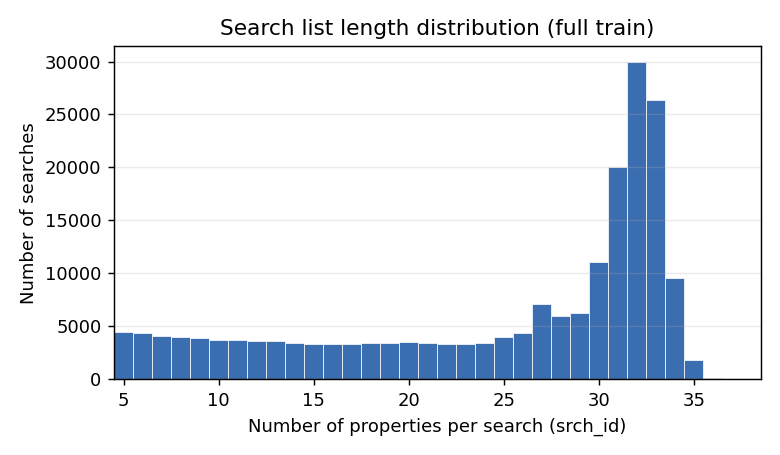
\includegraphics[width=0.78\linewidth]{figures/list_length.png}
\caption{Search-list length distribution on the full training set.
Bimodal: a flat low-frequency segment from length 5 to 25 and a
sharp peak at 30 to 33. Median 29.}
\label{fig:list-length}
\end{figure}

\begin{figure}[t]
\centering
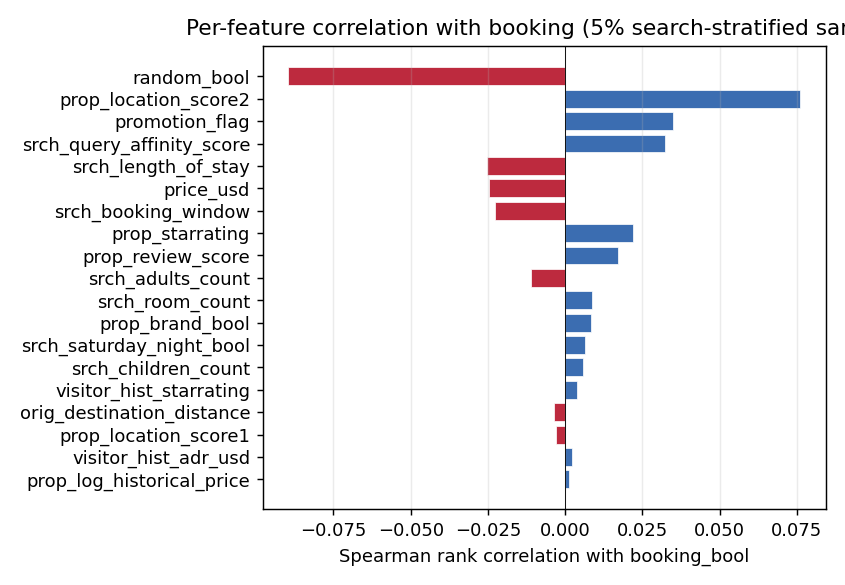
\includegraphics[width=0.78\linewidth]{figures/spearman_corr_with_booking.png}
\caption{Spearman rank correlations of numeric features with
\texttt{booking\_bool} on a five percent search-stratified sample.
The strongest absolute correlations are \texttt{random\_bool}
($-0.0896$) and \texttt{prop\_location\_score2} ($+0.0760$); all
other features sit below 0.04. No single feature can rank well on
its own.}
\label{fig:spearman}
\end{figure}

\begin{figure}[t]
\centering
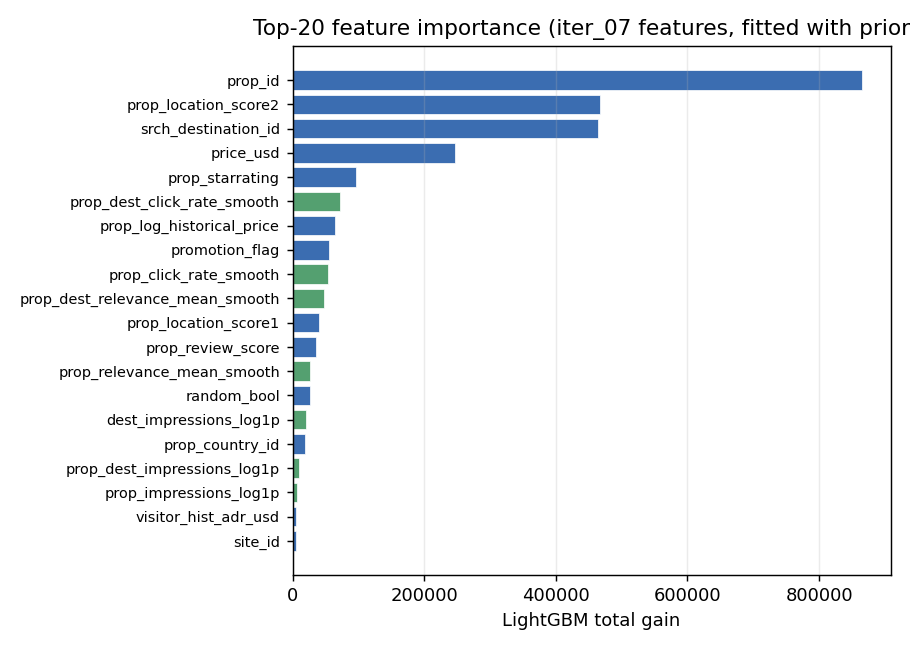
\includegraphics[width=0.78\linewidth]{figures/feature_importance_lightgbm.png}
\caption{Top-20 features by LightGBM total gain in a model fitted
on the 49 anchor features plus the 12 leakage-safe priors.
Categorical \texttt{prop\_id} dominates, followed by
\texttt{prop\_location\_score2}, \texttt{srch\_destination\_id},
\texttt{price\_usd}, and \texttt{prop\_starrating}; the strongest
prior feature \texttt{prop\_dest\_click\_rate\_smooth} ranks
sixth.}
\label{fig:importance}
\end{figure}

\section{Bias, deployment, and limitations}
\label{sec:bias-deployment}

\subsection{Bias detection}
\label{sec:bias-detect}

We segment the holdout along two dimensions and report NDCG@5 plus
exposure@5, which we define as the share of in-search positives
that surface in the top 5. By visitor country, the largest segments
land between 0.350 and 0.416 NDCG@5 with exposure close to 1.0;
the lowest score is for country 99 (0.349878 NDCG@5, exposure
0.9612). By property popularity tertile (computed from total
training impressions per \texttt{prop\_id}) the picture is
sharper: the high tertile reaches exposure 0.9266 with NDCG@5
0.390424, the medium tertile 0.2651 / 0.395074, and the low
tertile 0.2010 / 0.426924. The low tertile has the highest
per-search NDCG when those hotels appear; they simply do not
appear in the top 5 often. We therefore frame this as exposure
disparity, not as a discrimination claim: high-popularity
properties dominate the top of the ranking, and that visibility
gap propagates to future training data.

\subsection{Mitigation: post-processing exposure rerank}
\label{sec:bias-mitigate}

We mitigate with a single post-processing step. For each property
$p$ in popularity tertile $t(p)$ with prior probability
$P_{t(p)}$ on train, we rerank by
\begin{equation}
\tilde{s}(p) \;=\; s(p) \;+\; \lambda \cdot \bigl(-\log P_{t(p)}\bigr),
\qquad \lambda = 0.20 ,
\end{equation}
which leaves the original ranker score $s(p)$ untouched but adds
a tertile-prior penalty that grows for under-represented tertiles.
On the locked holdout, $\lambda = 0.20$ produces the trade-off in
Table~\ref{tab:bias-tradeoff}: a global NDCG@5 drop of 0.003090 buys a
5.3 percentage point gain in medium-tertile exposure and a 2.2
percentage point gain in low-tertile exposure. The high tertile
loses 3.0 percentage points. The primary Kaggle submission is
unmodified; the rerank is a deployment-time variant.

\begin{table}[t]
\centering
\caption{Popularity tertile exposure and NDCG@5 before and after
the post-processing rerank with $\lambda = 0.20$.}
\label{tab:bias-tradeoff}
\begin{tabular}{lrrrr}
\toprule
tertile & exposure before & exposure after & NDCG@5 before & NDCG@5 after \\
\midrule
high   & 0.9266 & 0.8965 & 0.390424 & 0.381779 \\
medium & 0.2651 & 0.3184 & 0.395074 & 0.422510 \\
low    & 0.2010 & 0.2227 & 0.426924 & 0.442720 \\
\bottomrule
\end{tabular}
\end{table}

\begin{figure}[t]
\centering
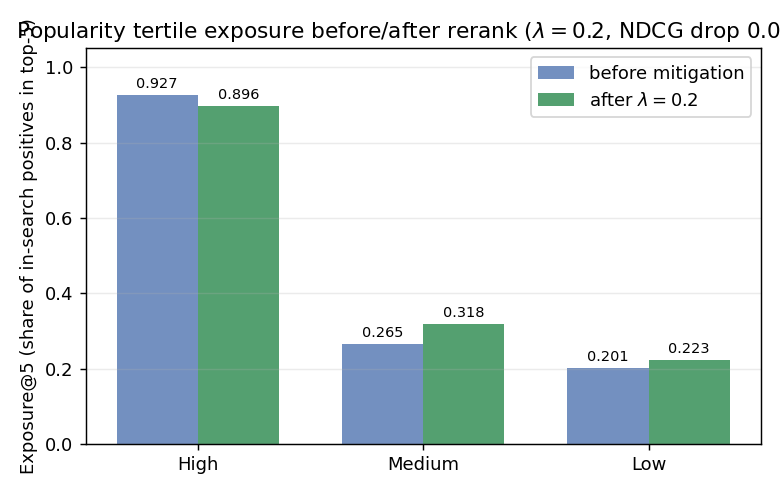
\includegraphics[width=0.72\linewidth]{figures/bias_exposure_before_after.png}
\caption{Popularity tertile exposure@5 before and after the
post-processing rerank with $\lambda = 0.20$ on the locked holdout.
The high tertile loses about 3 percentage points of exposure;
the medium and low tertiles gain about 5 and 2 percentage points
respectively. The corresponding global NDCG@5 drop is 0.003090.}
\label{fig:bias-exposure}
\end{figure}

\subsection{Honest local-to-public discussion}
\label{sec:shrinkage}

Across the verified Kaggle uploads the local-to-public gap moved
in one direction: Table~\ref{tab:shrinkage} shows the trajectory.

\begin{table}[t]
\centering
\caption{Local holdout NDCG@5 versus Kaggle public NDCG@5 for the
three uploaded submissions. Local holdout is on the locked split;
public is the Kaggle public leaderboard.}
\label{tab:shrinkage}
\begin{tabular}{lrrr}
\toprule
submission & local & public & gap \\
\midrule
Submitted safe baseline                & 0.395289 & 0.39500 & $+0.000289$ \\
Diverse ensemble submission            & 0.399638 & 0.39685 & $-0.002788$ \\
Historical-prior final submission      & 0.400682 & 0.39690 & $-0.003782$ \\
\bottomrule
\end{tabular}
\end{table}

The direction of improvement transferred (public moved from
0.39500 to 0.39685 to 0.39690), but the magnitude shrank: the
local-to-public gap of $+0.000289$ on the safe baseline became
$-0.003782$ on the final model. Each individual decision was
leakage-safe by construction (Group K-fold on \texttt{srch\_id},
no train-test joint statistics, locked holdout, fixed
\texttt{prop\_id} test set), but the cumulative exploratory budget
on the same locked holdout introduced a second-order optimism: we
kept whichever change scored highest on that fixed set, so the
expected public improvement was overstated. The reported public
0.39690 should be read as a verified outcome and not as a
prediction of the local 0.400682 transferring.

Anti-overfitting decision in the final exploratory stage: we
identified a rank-blend candidate (a holdout-max rank aggregation
variant, weighted 0.60 final + 0.30 diverse + 0.10 safe) that scored
0.401482 on the locked holdout, $+0.000800$ above the final selected
model. We did not select it. Selecting the holdout-max of a small
grid is exactly the move the shrinkage trajectory warns against; we
instead followed a pre-specified heuristic (simplest non-trivial
blend with at least two methods and holdout $\geq 0.398$) which
picked the conservative weighting at 0.400453, and we did not upload
that either. The headline submission remains the simpler historical-
prior 3-seed model.

\subsection{Deployment notes}
\label{sec:deploy}

We sketch a deployment pattern faithful to what the codebase
already supports.

\paragraph{Request-time scoring.}
For an incoming search the model receives the candidate property
list together with the search-context fields. Anchor features and
the 12 priors are computed per row. The K-fold encoding is
training-time only: at request time we use the full-train
aggregates (Section~\ref{sec:priors}), which is leakage-safe because
incoming searches are group-disjoint from training searches by
construction. Scoring is batched per search (groups of 5 to 38
properties), which fits comfortably in a single LightGBM
\texttt{predict} call.

\paragraph{Cold-start hotels.}
A new \texttt{prop\_id}, a new \texttt{srch\_destination\_id}, or
a new pair has zero impressions in train. The Laplace smoothing
in Equation~\ref{eq:smooth} reduces to $\bar{y}_{\text{global}}$ for those
keys, so the model still receives a sensible prior signal and
falls back to the raw anchor features (\texttt{price\_usd},
\texttt{prop\_starrating}, \texttt{prop\_location\_score1/2},
\texttt{promotion\_flag}). No separate cold-start path is needed.

\paragraph{Monitoring.}
We recommend tracking three families of metrics. (i) Offline
NDCG@5 monthly on a held-out slice with the same group-aware
protocol. (ii) Click and book rate on the served top-5 weekly,
since these are model-free proxies that catch obvious regressions.
(iii) Exposure@5 by popularity tertile and by visitor country,
weekly, with an alert if the high-tertile share rises above the
pre-mitigation level. The fairness-aware variant
($\lambda = 0.20$, Section~\ref{sec:bias-mitigate}) is an opt-in
deployment switch with a known NDCG@5 cost of 0.003090 on the
locked holdout.

\paragraph{Retraining cadence.}
Anchor features and the LightGBM model are retrained monthly on
the rolling training window. The 12 priors are refreshed on the
same cadence and recomputed per fold from the new training
window; we do not stream the priors at request time.

\paragraph{Limitations.}
Three limitations carry into deployment. First, the local-to-public
shrinkage in Section~\ref{sec:shrinkage} suggests holdout-based selection
loses calibration after many iterations; we recommend a single end-to-end
holdout run or nested cross-validation for any future evaluation pass.
Second, we did not validate the model on a stricter time-based
split, which would be the right protocol if test were genuinely in
the future; here train and test cover the same date range so
group-aware splitting is sufficient. Third, the bias evaluation
uses popularity tertiles and visitor country with adequate-support
thresholds (at least 500 searches and 100 positives per segment);
finer or intersectional segments are not reported.

\section{Conclusion}
\label{sec:conclusion}

A LightGBM LambdaMART model on 49 anchor features plus 12
leakage-safe historical priors reaches public NDCG@5 = 0.39690 on
this year's instance of the assignment. The path from a heuristic
floor at 0.2836 (locked holdout) to a verified public score of
0.39690 was driven by a small set of carefully ablated choices
(anchor feature design, label-gain calibrated to the assignment
relevance grades, score-averaged 3-seed ensembling, K-fold
group-safe historical priors). The path from the safe baseline at
0.39500 public to 0.39690 public was much smaller, and the local
gain shrank in transfer; we report the gap honestly. Two
extension directions that did not pay off (a holdout-max rank
blend and a fourth prior block keyed by visitor country) are
documented in the ablation table as negative results. The
deployment design supports a fairness-aware exposure rerank as an
opt-in switch with a measured NDCG@5 cost.

\bibliographystyle{splncs04}
\bibliography{references}

\end{document}
